%        File: survey.tex
%     Created: ven. mai 18 02:00  2018 C
% Last Change: ven. mai 18 02:00  2018 C
%
\chapter{State of the Art}
This section first gives the definition of clustering along with its use cases and its main difficulties. Then several commonly met methods are presented along with the category of algorithms they belong to. Eventually we focus on the specific subfield of multi-view clustering, giving a definition and a state of the art of the research works which are conducted on it.

    \section{Definition of clustering}
    Every day, exabytes of data of various format are generated: videos, texts, audio, activities on social networks\ldots Since its creation, clustering has become an active field of research because of the possibilities it offers when applied to such a variety of data. Using clustering, it becomes possible to better understand the underlying structures of a dataset. These structures can then be used for further real-world applications such as market study, advertisement targeting, product improvement and recommendation.

    In~\cite{jain1999data}, the clustering is defined as ``[\ldots] the unsupervised classification of patterns (observations, data items, or feature vectors) into groups (clusters)''. The term unsupervised refers to one of the two subfield of Machine Learning: supervised and unsupervised learning. A problem is said to be supervised if the learning algorithm is trained knowing both the input and the corresponding labels (classification for example). On the opposite, a problem is said to be unsupervised if one has only access to its input, which is the case of the clustering for which one has to define clusters only knowing input data.  

    The first two clustering algorithms found in the literature are Hierarchical Clustering~\cite{ward1963hierarchical} and K-means~\cite{macqueen1967some} respectively defined in 1963 and 1967. Those algorithms define two of the main clustering subfields: the methods based on a hierarchical classification of the input, and the methods based on its partition. The different clustering subfields will be described later in this section.

    \section{Results analysis}
    Clustering in itself is a very broad field, and it might be difficult to analyze the results of a training process depending on its context. Criterions usually met to analyze a clustering are detailed in this section: the similarity measures along with how they are related to data typology, then quality measures.
    
    \subsection{Similarity measures}
    The second problem related to clustering lies in the similarity measures used for each algorithm. Clustering relies on the idea that similar individuals must belong to the same cluster while dissimilar ones should not. Therefore, one of clustering challenges is to define the criterion that allows to compare two individuals. Problems such as point clustering in ``physical'' space can be adressed using distance measures among which the most well-known is the euclidean distance, a.k.a.\ the $l2$-norm and defined as follow: 
    
    \begin{equation}
    d\left(x,y\right) = \sum_{k=1}^D {\left(x_k - y_k\right)}^2
    \end{equation}

    Where D is the dimension of $x$ and $y$, and $x_k$ the $k$-th coordinate of $x$ in its feature space. This measure is intuitive because it refers to the concept of distance which we use everyday. However, even if it is intuitive and can give good results in lower dimensional spaces, it has its limitation when the number of dimensions increases. The choice of the inter-individuals distance must consider points such as the space dimensionality, the type of features used in the dataset, and even the goal of the clustering. A guide on this problem can be found in~\cite{domingos2012few}.

    Also, the choice of a measure defines data topology in the sense that it defines the shape of the clusters that may be found. The topology of data is also a criterion to consider when choosing a clustering method because some may (or not) be used for certain kind of topologies. The diagrams displayed in documentation of the Python package \textit{scikit-learn}\footnote{\url{http://scikit-learn.org/stable/modules/clustering.html}} present how some methods may or may not adapt to some topologies. For example, methods such as K-means based on $l2$-norm defines ball-shaped clusters. This may not give the expected result when considering data forming concentric circles for example.

    From now, every time the term ``neighbor'' will be used in this thesis, it will implicitly entail that a distance between individuals has been defined. The definition of this distance can be viewed as an additional parameter for every method using it.

    \subsection{Quality measures}
\label{sec:quality_measures}
    Another problem appears when one has applied the selected clustering method on its dataset: how can one measures the quality of a clustering? With a supervised problem such as classification, it is easy to determine the quality of the result by simply considering criterion such as the percentage of object well classified. You can even use this criterion during the learning phase to deduce update rules as in~\cite{vincent2010stacked}. However, the problem is different for clustering: most of the time you do not have access to a criterion which you can optimize during the learning process. If the problem only involves data in a visualizable space (between 1 and 3 dimensions), it is easy to visualize the data and to see if the created clusters are intuitively good. However, most of the time the problem involved have a dimensionality that is far higher than 3, making it hard to visualize graphically the content of each cluster. Some methods such as Principal Component Analysis~\cite{wold1987principal} and Locally Linear Embedding~\cite{roweis2000nonlinear} allow to give an estimated projection of the data (and of their corresponding clusters) in a visualizable space. Some work in the literature are solely dedicated to the definition of a clustering quality, like in~\cite{ben2009measures}.

    However, even if it is hard to give an intuitive measure of the quality of a clustering, two criteria are intuitively studied to get an idea of the clustering quality: its compactness, namely how close are the individuals from a same cluster, and its separability, namely how far are the individuals from different clusters.\ some measures allow to compare two clustering one to each other. Among these measures, the most commonly met are the Dunn index~\cite{dunn1973fuzzy}, the Davies-Bouldin index~\cite{davies1979cluster}, the Silhouette index~\cite{rousseeuw1987silhouettes} the Wemmert-Gancarski Index~\cite{wemmert2000classification}. Some measures even allow to compare two clusterings, namely the Rand index~\cite{rand1971objective} and its Adjusted version~\cite{hubert1985comparing}. The four first measures are based on the idea that clustering should minimize the distance between members of a same cluster (compactness) while maximizing distance between members of different clusters (separability), which corresponds to the intuitive goal that one may want to achieve when performing clustering.  While the four first make it possible to say that one clustering is ``better'' than the other, the two last only define the similarity between two clustering, without telling which one is the best. Each one is detailed in the following paragraphs.

    \subsubsection{Dunn index}
    The Dunn index is defined as the ratio between an inter-cluster measure $D$ and a measure of scatter $\Delta_i$. It is defined as follow:

    \begin{equation}
        DU = \frac{\min\limits_{i \neq j}D(c_i, c_j)}{\max\limits_{i \in [1..C]} \Delta_i}
        \label{eq:du_index}
    \end{equation}

    With $C$ the number of cluster. $D$ and $\Delta_i$ can be defined in different ways, creating each time a new version of the Dunn index. Here are presented the most used versions:

    \vspace{0.8cm}

    {\setlength{\extrarowheight}{10pt}%
    \begin{table}[h]
    \centering
    \begin{tabular}{ll}
    \multicolumn{1}{c}{$\mathbf{D(c_i, c_j)}$}                   & \multicolumn{1}{c}{$\mathbf{\Delta_i}$}                                   \\ [10pt] \bottomrule
    $\min\limits_{x \in c_1, y \in c_2} d(x, y)$                           & $\max\limits_{x, y \in c_i} d(x,y)$                                                       \\ [10pt] \bottomrule
    $\max\limits_{x \in c_1, y \in c_2} d(x, y)$                           & $\min\limits_{x, y \in c_i} d(x,y)$                                                       \\ [10pt] \bottomrule
    $d(\mu_i - \mu_j)$                                             & $\frac{1}{|c_i|}\sum_{x \in c_i}(x - \mu_i)$                               \\ [10pt] \bottomrule
    $\frac{1}{|c_1||c_2|}\sum\limits_{x \in c_1}\sum\limits_{x \in c_2} d(x, y)$ & $\frac{1}{|c_i| \times (|c_i| - 1)} \sum\limits_{x, y \in c_i, x \neq y} d(x, y)$ \\ [10pt] \bottomrule
    \end{tabular}
    \caption{Different set of distance inter-clusters and measure of scatter for the Dunn index}
\label{tab:all_dunn_index}
    \end{table}}

    \vspace{0.8cm}

    With $\mu_i$ the center of the $i$-th cluster defined as follow:

    \begin{equation}
        \mu_i = \frac{1}{|c_i|}\sum_{x \in c_i}x
        \label{eq:mui}
    \end{equation}

    \subsubsection{Davies-Bouldin index}
    Based on the same idea than the Dunn index, the Davies-Bouldin index is defined as follows:

    \begin{equation}
DB = \frac{1}{|C|}\sum_{i=1}^{|C|} \max_{j \neq i} \frac{\Delta_i + \Delta_j}{D(c_i,c_j)}
        \label{eq:db_index}
    \end{equation}

    With $C$ the clustering and $|C|$ the corresponding number of clusters, $\Delta_i$ a measure of scatter for the $i$-th cluster and $D(c_i, c_j)$ a distance measure as defined for the Dunn index. The most commonly met version of the Davies Bouldin index in the one based on the third line of Table~\ref{tab:all_dunn_index}.

    \subsubsection{Silhouette index}
    The Silhouette index (SI) can also be used to assess the compactness of the clusters as well as their separation. However, the main difference between this index and the Dunn or Dabies-Bouldin ones is that it can be computed either for a given individual $x$, or for a cluster $c_i$, or for the whole clustering. For an individual $x$, $a_x$ is defined as the mean distance between $x$ and the elements belonging to its cluster, and $b_x$ is defined as the mean distance between $x$ and the elements which do not belong to its cluster. Then, the Silhouette index in defined as follow:

    \begin{equation}
        SI(x) = \frac{b_x - a_x}{\max(a_x, b_x)}
        \label{eq:si_x}
    \end{equation}

    From which it follows that 

    \begin{equation}
        SI(x) = 
        \begin{cases}
            \frac{b_x}{a_x} - 1, & \text{if}\ a_x > b_x \\
            0, & \text{if}\ a_x = b_x \\
            1 - \frac{a_x}{b_x}, & \text{if}\ a_x < b_x \\
        \end{cases}
        \label{eq:si_x_detail}
    \end{equation}

    This implies that $SI(x)$ takes values between -1 and 1. A value near -1 means that the distance between $x$ and the element from its cluster is bigger than the one between $x$ and all the other elements, meaning that $x$ does not belong to the good cluster. On the opposite, if $x$ is near 1, it means that it is closer to the elements from its cluster, which may indicate that $x$ is in the right cluster. When this value is computed for every $x$ in a cluster, the SI of the cluster can be computed as follow:

    \begin{equation}
        SI(c_i) = \frac{1}{|c_i|}\sum_{x \in c_i} SI(x)
        \label{eq:si_ci}
    \end{equation}

    And eventually, when $SI(c_i)$ is computed for all the clusters, the SI of the whole clustering can be computed:

    \begin{equation}
        SI(C) = \frac{1}{|C|}\sum_{i=1}^{|C|} SI(c_i)
        \label{eq:si_clustering}
    \end{equation}

    If one would like to use this index, it has to be noticed that it is computationaly expensive to compute it. Even if an intermediary structure is used to store the distances already computed, the index will have to compute $\frac{1}{2}n(n-1)$ distances, with $n$ the number of elements in the dataset.
    
    \subsubsection{Wemmert-Gancarski index}
    The Wemmert-Gancarski (WG) index is another index based on the pair compactness-separability. It is defined as follow

    \begin{equation}
        WG(c_i) = 
        \begin{cases}
            0 ~ \text{if}\ \frac{1}{|c_i|}\sum_{x \in c_i} \frac{d(x,\mu_i)}{d(x, \mu_j)} > 1\\
            1 - \frac{1}{|c_i|}\sum_{x \in c_i} \frac{d(x,\mu_i)}{d(x, \mu_j)} ~ \text{otherwise}
        \end{cases}
        \label{eq:wg_index}
    \end{equation}

    This index takes its values between 0 (bad score) to 1 (good score). To get the result on a complete clustering, the following formula is applied:

    \begin{equation}
        WG(C) = \frac{\sum_{i=1}^{|C|} |c_i| WG(c_i)}{\sum_{i=1}^{|C|} |c_i|}
        \label{eq:wg_index_global}
    \end{equation}

    \subsubsection{Rand index}
    To compare two clustering, the Rand index considers the peers of elements which are clustered together (or not) in each clustering. Four sets are defined ($a$, $b$, $c$, and $d$), the union of which contain all the peers of elements of the dataset studied. The belonging of a pair to a set follows Table~\ref{tab:rand_index}.
    
    \vspace{0.8cm}

    \begin{table}[h]
    \centering
    \begin{tabular}{lcc}
                                       & \multicolumn{1}{l}{\textbf{Same cluster in $C_1$}} & \multicolumn{1}{l}{\textbf{Same cluster in $C_2$}} \\ \bottomrule
    \multicolumn{1}{l}{\textbf{$a$}} & yes                                                 & yes                                                 \\ \bottomrule
    \multicolumn{1}{l}{\textbf{$b$}} & no                                                  & no                                                  \\ \bottomrule
    \multicolumn{1}{l}{\textbf{$c$}} & yes                                                 & no                                                  \\ \bottomrule
    \multicolumn{1}{l}{\textbf{$d$}} & no                                                  & yes                                                 \\ \bottomrule
    \end{tabular}
    \caption{Sets of peers of elements used for the definition of the Rand index}
\label{tab:rand_index}
    \end{table}

    \vspace{0.8cm}

    Using these sets, the Rand index can be defined as follow:

    \begin{equation}
        RI(C_1, C_2) = \frac{a + b}{a + b + c + d} = \frac{a + b}{\binom{n}{2}} = \frac{2(a + b)}{n(n-1)}
        \label{eq:rand_index}
    \end{equation}

    The Rand index takes its values between 0 (totally different) and 1 (identical). A corrected version of the Rand index has been proposed in order to correct the possibility that two clusterings are equal because of randomness. This Adjusted Rand Index is defined as follow:

    \begin{equation}
        ARI(C_1, C_2) = \frac{\sum_{ij}\binom{n_{ij}}{2} - \big[\sum_i\binom{a_i}{2}\sum_j\binom{b_j}{2}\big]/\binom{n}{2}}{\frac{1}{2}\big[\sum_i\binom{a_i}{2} + \sum_j\binom{b_j}{2}\big] - \big[\sum_i\binom{a_i}{2}\sum_j\binom{b_j}{2}\big]/\binom{n}{2}}
        \label{eq:adj_rand_index}
    \end{equation}

    With $n_{ij}$ the number of elements in common between the $i$-th cluster of $C_1$ and the $j$-th cluster of $C_2$, $a_i = \sum_j n_{ij}$ and $b_j = \sum_i n_{ij}$.\\

    This multiplicity of criteria brings to light that there are several challenges to address while performing clustering, and there is to date no method which can tackle all of them at once. Thus, the methods which have emerged have their own strengths and weaknesses. The next section presents an overview of the most well-known clustering algorithms used today with their specificities.

    \section{Popular clustering methods}

    This section presents a non-exhaustive selection of clustering algorithms which are the most commonly met in practice. Since the creation of the field, many methods have been proposed, and some of them share basic ideas which are then developed in different ways. Thus this section will be divided following the main categories of existing algorithms with at least one example for each kind. These categories are the following:

    \begin{itemize}
        \item Hierarchical methods
        \item Vector quantization methods
        \item Density based methods
        \item Stochastic methods
        \item Other methods 
    \end{itemize}

    The categorization presented here only pretends to give to the reader an overview of the most commonly met clustering algorithms. Some other categorization may be found in the literature, as the one presented in~\cite{jain1999data}, in~\cite{xu2005survey} and most recently in~\cite{fahad2014survey}.

    \subsection{Hierarchical methods}

    This kind of algorithm is the first to appear in 1963 with the method presented in~\cite{ward1963hierarchical}. Its core idea is to build a hierarchy of clusters by joining existing clusters (agglomerative methods, each individual starts in its own cluster) or by separating them (divise methods, all the dataset belongs to the same initial cluster). The principle of the method is to iteratively build a dendrogram by looking at a specific criterion. A method is defined both by the way the dendrogram is built and by the criterion used to pair or divise the clusters. One can either applies the method until all points belong to the same cluster and graphically determining the best number of clusters, or applies the method until a specific criterion is reached (number of clusters or inter-cluster distance for example).

    The first most commonly met hierarchical clustering method is the Agglomerative method presented in~\cite{ward1963hierarchical} which pairs clusters by considering a criterion to optimize. The variations of the algorithm depends on the criterion which is used to pair the clusters. The most used criterions are the Ward's function (defined in~\cite{ward1963hierarchical}) which aims at minimizing the intra-cluster variance at each step, and the linkage functions which consider a specific distance inter-cluster to minimize. These latter can be either the maximum or the minimum or the mean distance between points of two clusters (respectively called the complete-linkage, the single-linkage and the average linkage clusterings). There exists some other criterion which are not detailed here, however the interested reader can refer to~\cite{murtagh1983survey} which establishes a detailed survey on the criterion used for Agglomerative clustering. A general framework for an agglomerative hierarchical clustering algorithm is presented in Algorithm~\ref{alg:hierarch}.\\

    \begin{algorithm}[H]
        \caption{General framework of a hierarchical agglomerative clustering algorithm}
        \textbf{Initialization:} Create a cluster for each element\\
        Each cluster becomes a leaf for the dendrogram\\
        \While{there is more than one cluster left}{
            Compute pairwise inter-clusters similarities\\
            Merge the two most similar clusters\\
            Update the dendrogram
        }
        Cut the dendrogram to get the desired number of cluster
\label{alg:hierarch}
    \end{algorithm}

    \vspace{0.8cm}

    The second most commonly met Hierarchical method is the Balanced Iterative Reducing and Clustering using Hierarchies (BIRCH) one~\cite{zhang1997birch}. This method has been defined in a context of growing interest for data mining of large dataset, and its main claim is to reduce the consumption of ressources used during the clustering, as it presents a compact representation of a dataset and only requires a single pass through the dataset to create the tree.

    \subsection{Vector quantization methods}
\label{sec:cluster_vector_quantization}

    Vector quantization methods are based on the idea that a clustering can be summarized by a set of prototype vectors, thus the belonging of an individual to one cluster is determined by comparing it to the set of existing prototypes. There are two main kinds of Vector Quantization methods: these based on deterministic belongings for which an individual belong to one and only one cluster, and these based on stochastic belongings for which belongings are expressed as a set of probabilities, one per prototype. 

    The Deterministic Vector Quantization methods are historically the first ones that have been created. The very first method, still used today, is the K-means algorithm~\cite{macqueen1967some}. This method is based on a pair of steps done iteratively until convergence of the prototypes. First a set of $K$ prototypes is randomly generated in the feature space, then each individual is associated with its closest prototype (in terms of a distance criterion). When all the dataset has been processed, the prototypes are updated as the means of their associated individuals: they become the ``center'', also called ``centroid'',  of the cluster they represent. The last two steps are repeated until the prototypes updates norms are sufficiently small to be considered as negligeable. The k-means algorithm is illustrated in Algorithm~\ref{alg:kmeans}.

    \begin{algorithm}
        \caption{K-Means algorithm}
\label{alg:kmeans}
        \textbf{Initialization:} Choose a value for $K$\\
        Randomly initialize the $K$ centroids $\mu_i$\\
        \While{a stopping criterion is not met}{
            \ForAll{$x_n \in X$}{
                Assign $x_n$ to the cluster $c_i$ with the closest centroid\\
                $s_{n,i} = 
                    \begin{cases}
                        1 \quad \text{if} \quad i = argmin_i\|x_n - \mu_i\|^2\\
                        0 \quad \text{otherwise}
                    \end{cases}$
            }
            \ForAll{$\mu_i$}{
                $\mu_i = \frac{\sum_n x_n \cdot s_{n,i}}{\sum_n s_{n,i} }$
            }
        }
    \end{algorithm}

 The initial method has allowed the emergence of many variations such as k-medians clustering~\cite{jain1988algorithms}, k-medoids clustering~\cite{kaufman1987clustering} depending on the prototype update rule. An extension to this algorithm has been proposed in~\cite{kohonen1998self} in which the authors define the Self-Organizing Maps (SOM). This methods is based on the same idea than K-means, except that the prototypes are organized as a map in which each node update will also impact its neighbors, depending on a neighboring function based on the Manhattan distance between two nodes in the map. The Manhattan distance between two neurons in a SOM is defined as the minimum number of hops separating the two nodes in the map. This allows to not only capture prototypes, but also to organize them following a possible underlying structure in the dataset. This method also makes possible to get a two or three dimensional representation of a possibly high feature space. Indeed in a supervised case, by assigning to each node the class of the majority of its associated individuals, it it possible to graphically see the underlying proximity structure in the dataset. 

A SOM is defined by a temperature function $\lambda$ which itself defines a neighborhood function $K$. The temperature function is usually defined as follow:

    \begin{equation}
    \lambda(t) = \lambda_{\min}{\Big(\frac{\lambda_{\max}}{\lambda_{\min}}\Big)}^{\frac{1}{t}}
        \label{eq:som_temp}
    \end{equation}

    With $\lambda_{\min}$ and $\lambda_{\max}$ two parameters of the SOM algorithm defining the minimum and maximum temperature used during the training. One can notice that the function goes from $\lambda_{\max}$ for $t=1$ to $\lambda_{\min}$ for $t\to \infty$. This function is then used to define the following neighborhood function:
    
    \begin{equation}
        K_{k,l} = \exp\Big(-\frac{d^2(k,l)}{\lambda(t)}\Big)
        \label{eq:som_neigh}
    \end{equation}

    The idea behind this function is to determine the width of the neighborhood affected by the modification of a single neuron. The higher $\lambda(t)$, the hotter is said the map, and the wider is the neighborhood impacted by the modification of a neuron. However, this wider area comes with a limitation in the modification that can be performed on each neuron. This phenomenon is related to the exponential function used for $K$, if the map is hot, the map performs global modifications of its structure in order to adapt to the data typology. On the opposite, when the map is cold, the map only performs local modifications in order to adapt its neuron to its immediate neighborhood.

    A description of the SOM algorithm is presented in Algorithm~\ref{alg:som}.

    \begin{algorithm}
        \caption{SOM algorithm}
\label{alg:som}
        \textbf{Initialization:} Choose the dimensions $n \times m$ of the map\\
        Randomly initialize the $n \times m$ neurons $w_i$\\
        \While{a stopping criterion is not met}{
            \ForAll{$x \in X$}{
                Assign $x$ to its closest neuron $w_i$\\
                $X_i \triangleq$ set of all $x$ assigned to $w_i$
            }
            Compute $\lambda$ using Equation~\ref{eq:som_temp}\\
            \ForAll{$w_i$}{
                \ForAll{$w_j$}{
                    Compute $K_{i,j}$ using Equation~\ref{eq:som_neigh}
                    $w_j^{new} = w_j^{old} + \varepsilon K_{i,j} \sum_{x \in X_i} ( x - w_i )$
                }
            }
        }
    \end{algorithm}

 Deterministic Vector Quantization ideas have been adapted in a stochastic context: now, an individual does not belong to a single cluster, but rather is defined by a set of $K$ belonging probabilities, with $K$ the total number of clusters. The belongings are told to be ``fuzzy''. A comparision can be made between the two learning steps used by K-means and the Expectation-Maximization (EM) algorithm defined in~\cite{dempster1977maximum} for which the update of parameters are performed using the likelihood of data being generated by the model using these parameters. In the first case, the method optimizes the variance of the distance between the prototypes and its associated points, in the second case the method optimizes the likelihood of the dataset being generated by the clustering model. The EM method thus makes it possible to define a stochastic counterpart to K-means called Gaussian Mixture Model. In this method, data have been generated by a set of Gaussian functions. The EM method here make it possible to learn the mean, the variance and, in the multidimensional case, the covariance matrix of the functions.
    
 Considering fuzzy belongings, it is also possible to draw some links between deterministic clustering methods and their stochastic variants. Thus, Fuzzy C-Means~\cite{bezdek1984fcm} can be viewed as the stochastic variant of K-means for which the optimized criterion uses weighting coefficients equals to the fuzzy belongings defined by the method. Beside, the Generative Topographic Maps (GTM)~\cite{bishop1998gtm} can be viewed as the SOM stochastic variant. However, while Fuzzy C-Means (FCM) only added the stochastic belongings to the initial model, GTM uses the concept of latent space to define the prototype map, map which is then mapped into the feature space using a transformation which parameters are trained using the EM method (cf. Figure~\ref{fig:gtm}). A detailed description of the FCM algorithm can be found in Algorithm~\ref{alg:fcm}

        \vspace{0.8cm}
   
        \begin{figure}[h]
            \centering
            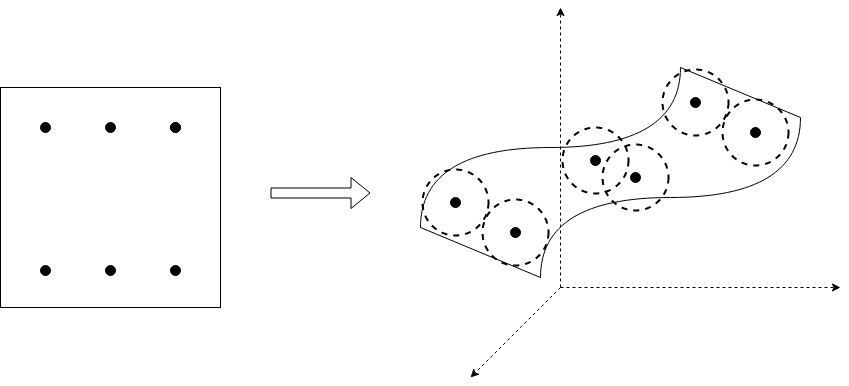
\includegraphics[scale=.3]{gtm}
            \caption{Generative Topographic Maps: projection of a map from the latent space to the feature space}
\label{fig:gtm}
        \end{figure}

    \begin{algorithm}
        \caption{Fuzzy C-Means algorithm}
\label{alg:fcm}
    \textbf{Initialization:} Choose a value for $C$ and $m$\\
    Randomly initialize $s^0_{n,i}$ such that\\
    $\forall i, ~ s_{n,i} \in [0,1], \quad \forall n ~ \sum\limits_{i=1}^C s_{n,i} = 1$\\
    r = 0
    \Do{a stopping criterion is not met}{
        \ForAll{$\mu_i$}{
            $\mu_i = \frac{\sum_n x_n {\left(s_{n,i}^{r-1}\right)}^m}{\sum_n x_n {\left(s_{n,i}^{r-1}\right)}^m}$
        }
        \For{$n\in [1..N]$}{
            \For{$i \in [1..C]$}{
                $s_{n,i}^r = \sum_{j=1}^C{\Big( \frac{d{(x_n, \mu_i)}^2}{d{(x_n, \mu_j)}^2} \Big)}^{-\frac{2}{m-1}}$
            }
        }
        $r = r+1$
    }
\end{algorithm}

These methods are further developed in Section~\ref{sec:soa_cc} when Collaborative Clustering is presented.

\subsection{Density based methods}

Even though hierarchical and vector quantization methods have been investigated since the emergence of clustering, the problem of the initialy defined number of cluster remains because it has to be defined manually by the user. The density-based methods presented in this section present alternative solutions to this problem by using the density of individuals in the feature space to automatically determine the optimal number of clusters during the learning process (w.r.t.\ the optimized criterion). This kind of method can also be seen as an intuitive answer to the clustering problem given the definition of a cluster: these methods are based on the finding of dense zones in the middle of less dense zones.

The most commonly met density based method is called Density-based spatial clustering of applications with noise (DBSCAN)~\cite{ester1996density}. Its core idea is to consider the density around each individual, namely their numbers of neighbors, because a cluster can also be seen as a densely populated point in the feature space. To do so, the method requires two parameters: a distance $varepsilon$ which determines if two points are neighbors, and $minPts$ which determines if an individual should be considered as a core sample (intuitively, a sample near the cluster center) or a non-core sample (at the fringe of the cluster, where the space is less densely populated). Starting from a random point, then iteratively: if it has at least $minPts$ neighbors, it is considered as a core point and all individuals such as their distances to the original point is less than $varepsilon$ are analyzed. If it has less than $minPts$ neighbors: either it has a core sample in its neighborhood, in which case it is considered a non-core sample belonging to the same cluster as its core neighbor, or in the opposite case, it is considered as an outlier belonging to no cluster. By doing so, the method defines its own number of clusters depending on $varepsilon$ and $minPts$. A description of the DBSCAN algorithm can be found in Algorithm~\ref{alg:dbscan}. The OPTICS algorithm~\cite{ankerst1999optics} can be seen as an improvement of the DBSCAN algorithm. This algorithm is based on both the ordering of the individuals in such a way that spatially close points become neighbors in the ordering and on the storage in each point of a distance used to define same cluster belongings. These points are used to address one of DBSCAN's weaknesses: the problem of detecting meaningful clusters in data of varying density.

\begin{algorithm}
    \caption{DBSCAN algorithm}
\label{alg:dbscan}
        \SetKwProg{Fn}{Function}{:}{}
        \SetKwFunction{FDBSCAN}{DBSCAN}
        \SetKwFunction{FexpandCluster}{expandCluster}
        \SetKwFunction{FregionQuery}{regionQuery}

        \Fn{\FDBSCAN{$X$,$\varepsilon$,minPts}}{
            $C=0$\\
            \ForAll{$x_n\in X$}{
                \If{$x_n$ has not been visited yet}{
                    mark $x_n$ as $visited$
                }
                $V_n$ = regionQuery ($x_n$,$\varepsilon$)\\
                \If{sizeOf ($V_n$) $\geq$ minPts}{
                    $C = C + 1$\\
                    expandCluster ($x_n$, $V_n$, $C$, $\varepsilon$, minPts)
                }
                \Else{
                    mark $x_n$ as noise
                }
            }
        }
        \Fn{\FexpandCluster{$x_n$, $V_n$, $C$, $\varepsilon$, minPts}}{
            Add $x_n$ to cluster $C$\\
            \ForAll{$x_i \in V_n$}{
                \If{$x_i$ has not been visited}{
                    $V_i$ = regionQuery ($x_i$, $\varepsilon$)\\
                    \If{sizeOf ($V_i > minPts$)}{
                        $V_n = V_n \cup V_i$
                    }
                }
                \If{$x_i$ does not belong to any cluster yet}{
                    Add $x_i$ to cluster $C$
                }
            }
        }
        \Fn{\FregionQuery{$x_n$, $\varepsilon$}}{
            list = $\emptyset$
            \ForAll{$x_i \in X$}{
                \If{$i \neq n$ and $d(x_n, x_i) \leq \varepsilon$}{
                    list = list $\cup ~ \{x_i\} $
                }
            }
            \KwRet{list}
        }
    \end{algorithm}


    The second most commonly met density based algorithm is the Mean-shift method defined in~\cite{cheng1995mean}. The core idea of the method is to consider individuals as mobile points which will then be attracted iteratively by high-density zones in the feature space. It is based on a kernel function $K$ which will define the attraction of a point on its neighborhood. At each iteration, each individual will be updated as the mean of its neighbors weighted by their respective attractions (defined by $K$). The method is entirely defined by the kernel function and by its parameters.

    \subsection{Special case: Spectral clustering}

    In this subsection we present the method called Spectral clustering and defined in~\cite{Ng01onspectral}. It is not presented in one of the previous sections because its core idea does not fit with these already defined, but also because it is made of two steps, one to reduce the problem dimensionality, and the second one to effectively cluster the dataset. The second step can be done using by any algorithm defined previously. The core idea of this method is to use the eigenvalues of a similarity matrix computed on the dataset to reduce the dimensionality of the future space using the associated eigen-vectors.


    \section{Collaborative Clustering}
\label{sec:soa_cc}

    \subsection{Multi-view learning}

    Methods presented so far rely on the learning of a whole dataset. However, it is possible to find cases in real life for which one does not have access to the totality of the dataset, because of privacy constraint for example (see Section~\ref{sec:crs_context} for further explanation). It is also possible that data may come from different heterogeneous sources. Both cases make the training of a single algorithm on the whole dataset difficult. This acknowledgment had led to the definition of a new clustering context, called the Multi-View Learning. In this context, many methods have to be trained together before being combined in order to achieve the goal initially set.
    
    As presented in~\cite{sun2013survey}, Multi-View Learning is a vast domain with many related subfields such as dimensionality reduction, semi-supervised, supervised learning and active learning. However, the following section is only focused on the application of Multi-View Learning in a clustering context, namely the collaborative clustering paradigm.
    
    \subsection{Cooperative versus Collaborative Learning}
    In the context of multi-view clustering, the methods proposed in the literature present solutions to two main problems:

    \begin{enumerate}
        \item Improve a global clustering knowing the clusterings performed on each view.
        \item Making the views collaborate to achieve a global inter-views consensus.
    \end{enumerate}

    As defined in~\cite{cornuejols2018collaborative}, the first subfield corresponds to Cooperative Clustering while the second one is called Collaborative Clustering. While these fields may seem closely related, their fundamentals differ in some points.

    Cooperative Clustering aims at making several clusterings of the same dataset by several different clustering methods. When each training is finished, the results are sent to a supervisor which task is to find a consensus between all the possible clusterings. Each training is done without inter-views communication, and the results are shared only during the final consensus phase performed by the supervisor. This consensus is found using different combination methods, as presented in~\cite{kittler1998combining,dietterich2000ensemble}. Several methods have been presented in the literature, the most known and used being Bayesian averaging~\cite{kittler1998combining}, Bagging~\cite{breiman1996bagging} and Boosting~\cite{freund1997decision}.

    Knowing this, Collaborative Clustering differs in many points from its Cooperative counterpart, the most important one being its final goal: while Cooperative Clustering aims at finding the best consensus among a set of clustering, Collaborative clustering aims at improving each local clustering knowing the results currently achieved by each other view. Moreover, the datasets used in each views do not have to be the same, this way Collaborative Clustering can work on heterogeneous data. Another difference lies in the inter-views communication: while each training was conducted independently with Cooperative Clustering, here each view has to communicate its intermediate results to its peers in order to improve each local result all along the training.
    
    From now, the remainder of this manuscript is focused only on the Collaborative Clustering.

    \subsection{Horizontal and Vertical}
\label{sec:cc_hor_ver}

    As previously presented, the goal of Collaborative Clustering is to make several views collaborate using their local results in order to achieve a better consensus. This general idea has two different declinations, depending on the similarities that the datasets have to share. These paradigms have been defined in~\cite{pedrycz2005knowledge} and in~\cite{grozavu2010topological}.

    If all the datasets contain different individuals represented by the same set of features, the collaborative clustering is called vertical. On the opposite, if all the datasets contain the same set of individuals described by different sets of features, the clustering is called horizontal (cf Figure~\ref{fig:hor_cc}).
    
    A third paradigm, called hybrid, is a combination of the two previously mentioned. In the work presented here, we have been interested in the horizontal version of Collaborative Clustering because it makes possible to tackle the problem of heterogeneous data coming from different sources, a problem that more and more applications are trying to deal with. The related works presented in the next Section are all related to horizontal clustering, unless the opposite is explicitly mentionned.
    \vspace{.8cm}

        \begin{figure}[h]
            \centering
            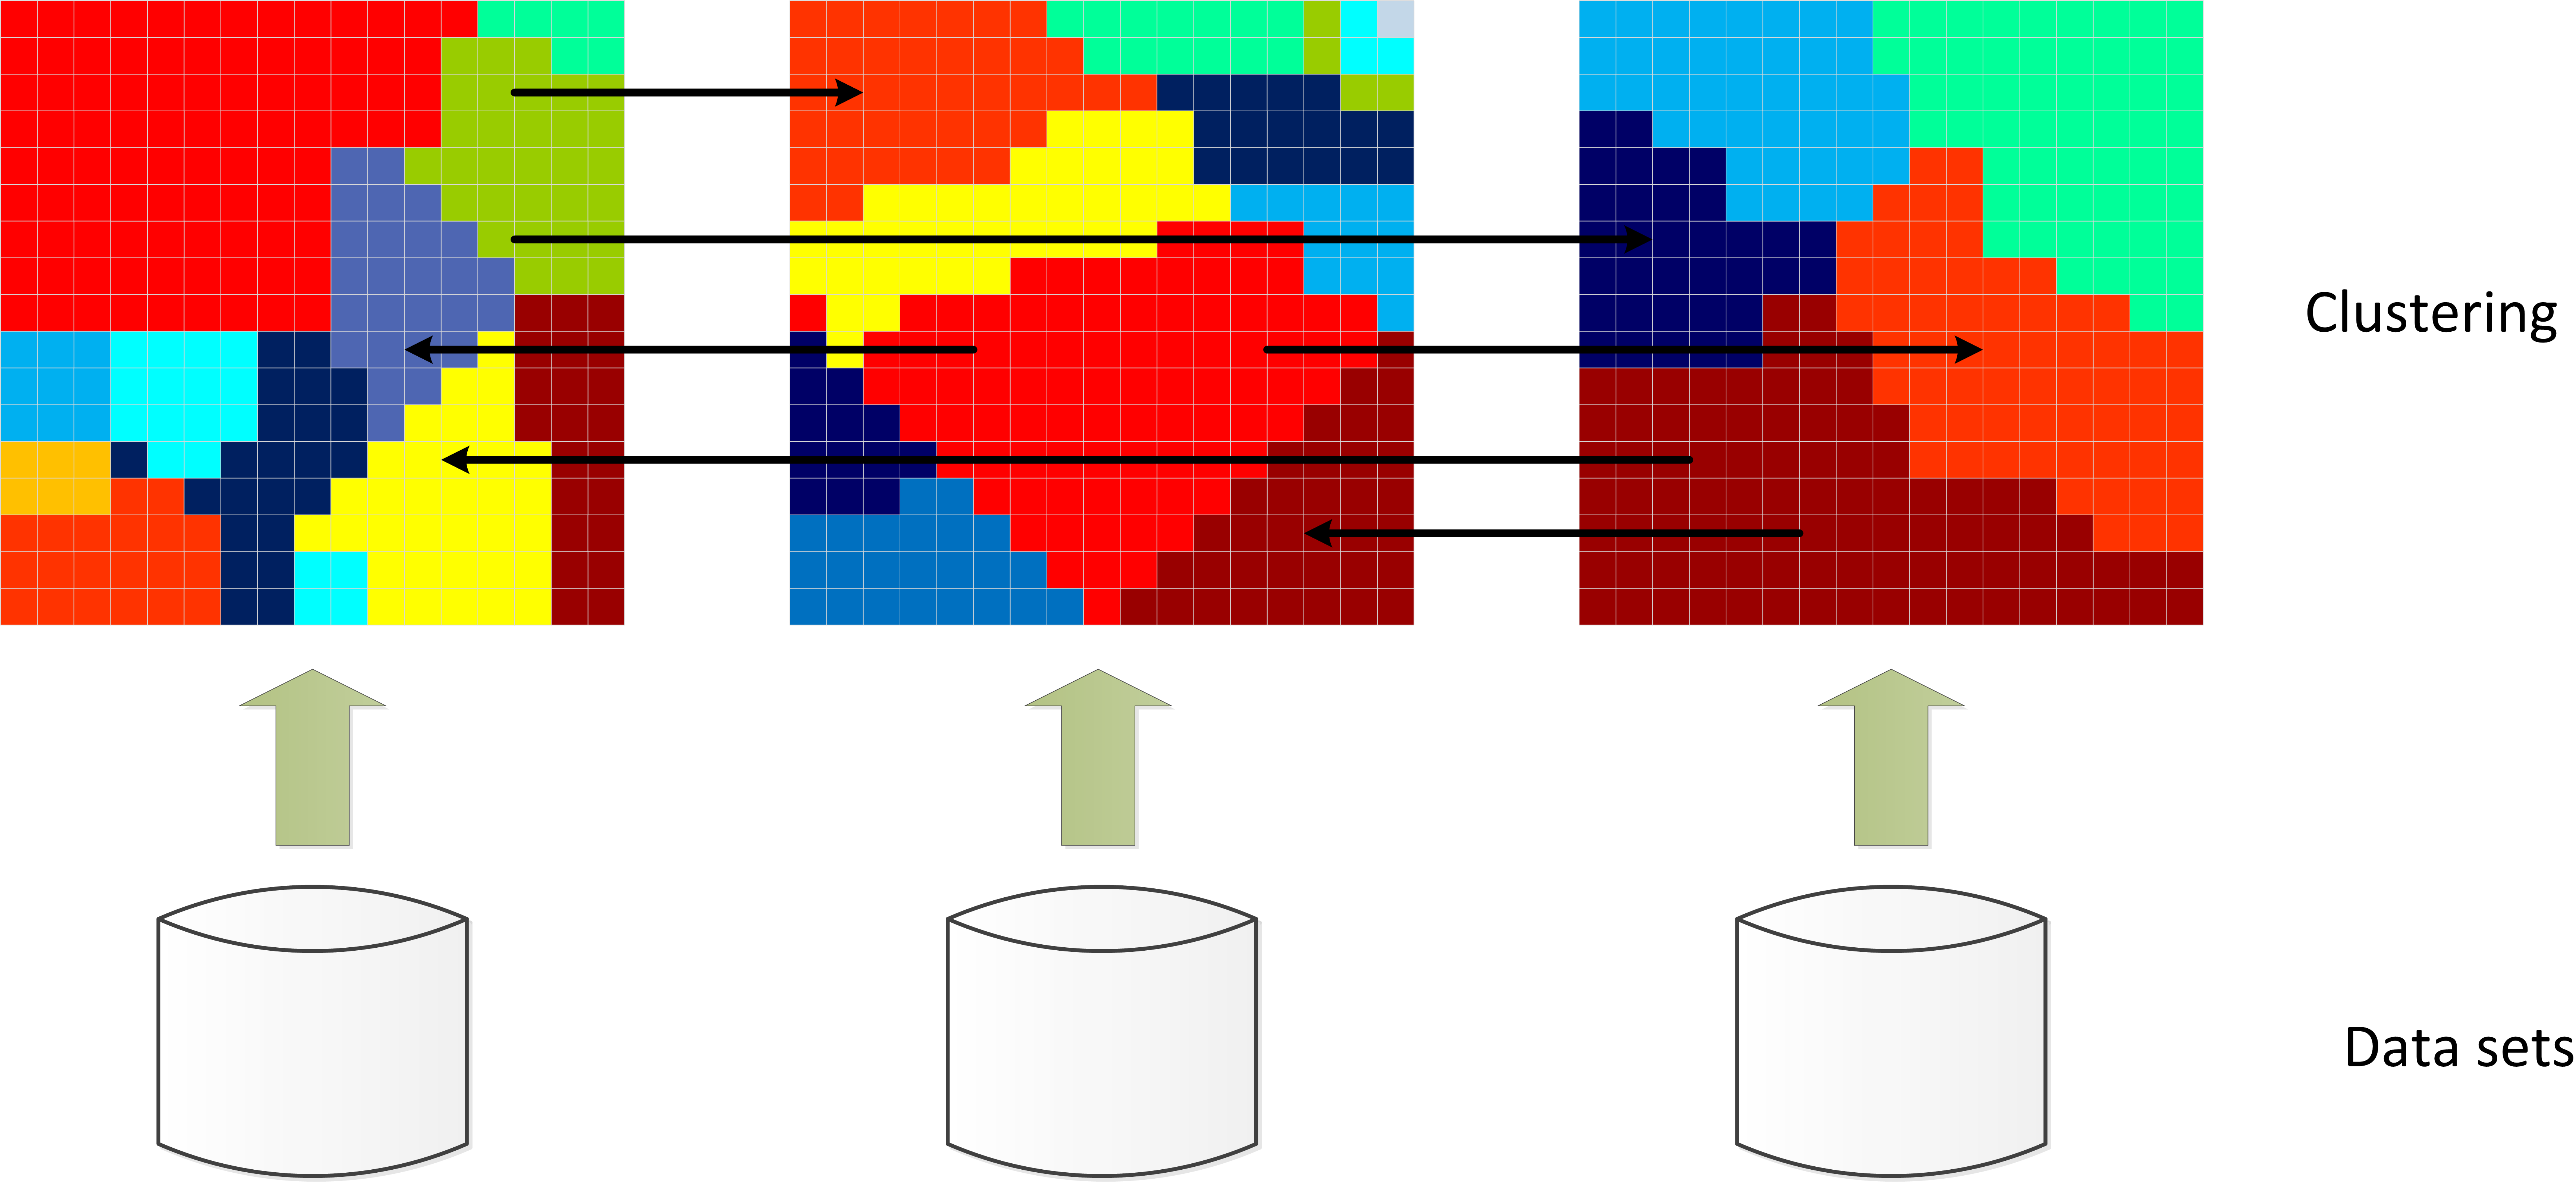
\includegraphics[scale=0.2]{hcc}
            \caption{Horizontal Collaborative Clustering}/
\label{fig:hor_cc}
        \end{figure}

    \subsection{Theory and Gradient Descent}
\label{sec:theo_grad_desc}
    
    Collaborative Clustering methods are based on two distinct phases introduced in~\cite{pedrycz2002collaborative}: a first phase of local clustering, during which each view produces a model of its data independently of the other views, and a second called collaborative during which the views exchange the information they have acquired during the first phase in order to continue to learn from what their peers have found. These two steps are the first theoretical parts defining a Collaborative Clustering method.

    Moreover, in Machine Learning, a method is usually designed around a function to optimize, called either cost function or criterion or even score. Collaborative Clustering consists in several algorithms collaborating, so each one has its own score to optimize. To formalize this idea mathematically and conjointly with the definition of the two steps mentioned above, two cost functions are computed per view.

    The first one is the usual cost function of the local methods used in each view. During the first local phase, each method produces a model according to this function. The second one takes into consideration the information learned by each view to formalize the idea of consensus between the views. Formally, the criterion of the $i$-th view can be written as follow:

    \begin{align}
        \label{eq:globalC}
        Q^i &= \alpha_i Q^i_{local}(V_i) + Q^i_{collab}(V_i, V_{j\neq i})\\
        &= \alpha_i Q^i_{local}(V_i) + \sum_{j\neq i} \beta^i_j C_j^i(V_i, V_j)
    \end{align}

    With $Q^i_{local}$ being the local criterion used to trained the local model of the $i$-th view, and $Q_{collab}$ being a term appended to the local criterion to formalize the collaborative part of the training. This latter term is made of the $N-1$ terms $C_j^i$ corresponding to a dissimilarity measure between the local views and its peers. $V_i$ stands for $i$-th view, and from now, we define $N$ as the total number of views. The coefficients $\alpha$ and $\beta$ are used to weight the relative importance of each term. Their definition is discussed later in this thesis.
    
    A summary on collaborative methods is given in the next Section. When the cost function is defined, its differentiate is computed and then used to generate rules to update the parameters of the system using gradient descent which generic formula can be written: 
    
		\begin{equation}
            {w}^{new} = {w}^{old} - \epsilon \, \frac{\partial E}{\partial w}
		\end{equation}
		
        where $\epsilon > 0$ is the parameter defining the learning rate of the process, $w$ the parameter to update, and $E$ the criterion to optimize. This update process is performed on every parameter $w$ until convergence. In practice, the learning is stopped when the norm of the update goes under a threshold fixed by the user. 
    
    \subsection{Existing approaches}

    \subsubsection{Fuzzy C-Means}

    Historically, the first version of Collaborative Clustering has been presented in~\cite{grozavu2010topological} and in~\cite{pedrycz2004fuzzy} and is based on Fuzzy C-Means~\cite{bezdek1984fcm}. During the local training phase, the method is using the following cost function:

    \begin{equation}
    \forall j \in [1..N], \quad Q^i_{local} = \sum_{n=1}^{|V_i|}\sum_{k=1}^C{(s_{n,k}^i)}^2|x_n - \mu_k^i|^2
        \label{eq:local_fcm}
    \end{equation}

    With $s_{n,k}^i$ being the probability the sample $n$ belongs to the $k$-th cluster, also called responsibility, $\mu_k^i$ the center of the $k$-th cluster, and $|\cdot|$ being the distance between two individuals. After the local training, the collaborative phase is performed: each view exchanges its responsibility matrix $S = (s_{n,k})$ with its peers. During this phase, each view has to minimize the following function:

    \begin{align}
        \forall j \in [1..N], \quad Q^i &= Q^i_{local} + Q^i_{collab}\\
    &= Q^i_{local} + \sum_{j\neq i}^N \beta^i_j\sum_{n=1}^{|V_i|}\sum_{k=1}^C{(s_{n,k}^i - s_{n,k}^j)}^2|x_n-\mu_k^i|^2
    \end{align}
    
    with $\beta^i_j$ being a weight defining the importance that view $i$ gives to the information coming from the external view $j$. The objective of the collaborative term of this function is to formalize the distance between the allocation vector of each sample. To better understand the use of this term, it is necessary to observe its behaviour in two extreme cases: when the responsibilities are roughly equal and when they are not. If all the responsibilities are approximately equal for two views, their respective clusterings are approximately equivalent, meaning that a consensus has been found, thus the collaborative term and the cost function are low. On the opposite, if the responsibilities are totally different, the sum of each absolute difference makes the term important, and so improvable. By considering these two cases, one can understand that the final goal of the horizontal collaborative clustering is to find the best consensus as possible between all the views.

    \subsubsection{Self Organizing Maps}
\label{sec:survey_som}

A second version of collaborative clustering has been proposed using self organizing maps~\cite{kohonen1998self}. It is based on the same idea as previously defined (FCM case), and has been presented in~\cite{grozavu2010topological}. Both collaborative and local terms are defined using $K_{k,l}$:

    \begin{equation}
        Q_{local}^i = \alpha_i \sum_{n=1}^{|V_i|}\sum_{k=1}^C K^i_{k,\chi(x_n)}\|x_n^i - w^k \|^2 
        \label{eq:som_cc_local}
    \end{equation}

    \begin{equation}
        Q_{collab}^i = \sum_{j \neq i}\beta_i^j \sum_{n=1}^{|V_i|}\sum_{k=1}^C \big(K^i_{k,\chi(x_n)} - K^j_{k,\chi(x_n)}\big)\|x_n^i - w^k \|^2 = \sum_{j \neq i} \beta_i^j C_i^j 
        \label{eq:som_cc_collab}
    \end{equation}

    With $d(k,l)$ being the Manhattan distance (number of hops) between the neurons $k$ and $l$ in the SOM, $\alpha_i$ being the weighting coefficient for the local view $i$, $\chi(x)$ being the function returning the closest neuron of $x$, and $w^k$ is the $k$-th neuron of the SOM.\@

    The learning process is the same as the one of the FCM version: first, each local view learns a model of its data using the standard SOM algorithm, then the neurons are updated during the collaborative phase following the cost function defined by~\ref{eq:som_cc_local} and~\ref{eq:som_cc_collab}.

    The collaborative clustering has also been applied using the Generative Topographic Mapping~\cite{bishop1998gtm} presented is Section~\ref{sec:cluster_vector_quantization}.

    \subsubsection{Generative Topographic Mapping}

    The GTM being considered as the stochastic evolution of the SOM, the use of the former as the local clustering method for Collaborative clustering instead of the latter has naturaly been studied and has been presented in~\cite{ghassany2012collaborative},~\cite{sublime2015vertical},~\cite{sublime2015horizontal} and~\cite{sublime2016collaborative}. The learning algorithm relies on the same principle as the SOM-based one, but this time using the Expectation-Maximization algorithm~\cite{dempster1977maximum}. During the Expectation phase each individual is assigned to a neuron. Then during the Maximization phase, the neurons are updated using a penalized likelihood as described in~\cite{green1990use}.\\

    \subsection{Genericity of Collaborative Clustering}
\label{sec:survey_limitations}

    The methods presented so far all share several limitations. First of all, the same algorithms have to be used in each view to make the collaboration possible. Moreover, because these algorithms are prototype based and because the collaboration phase relies on a comparison between the prototypes, the number of these prototypes has to be the same among all the views. An even more important restriction is that the maps defined by the SOM and the GTM algorithms have to be close to each other in order to be compared. Additionally, these methods rely on the weighting coefficients $\alpha$ and $\beta$ in order to select what collaborator should be favored or not during the learning process. These parameters have to be chosen carefully, and this may become a tricky task if many views have to be considered.

    Hopefully, several works have been conducted in order to remedy this situation. In~\cite{grozavu2014diversity} and in~\cite{rastin2015collaborative}, the impact of the diversity of the solution found by each local view on the collaboration is studied. Even if these work do not provide a way to automatically update $\alpha$ and $\beta$, it gives an intuition of what is important for a specific view when considering its external peers. An automatic update of the collaborative weights is presented in~\cite{grozavu2010topological} and in~\cite{grozavu2011learning}, also based on the gradient descent. However, this method still presents a significant constraint ($\beta = \alpha^2)$, which considerably simplifies the update of the weight to the detriment of the genericity of the method. In a recent article, a new entropy-based method is presented~\cite{sublime2018optimizing} having the double advantage to present a generic method to update the weighting coefficients $\beta$ ($\alpha$ not being used in this method) while being usable for any combination of local clustering method. This has been made possible because of the sharing of the results of each clustering (either deterministic or stochastic) instead of an intermediary information such as the neighborhood functions for the SOM.\@ This work is based on the researches previously presented in~\cite{sublime2016contributions}.

    \section{Conclusion}

    Through this state of the art, several improvable points have been identified. These points establish the guiding lines of the work presented in this thesis.

    First, one can notice the absence of incremental collaborative clustering methods among these previously presented. Now that Collaborative Clustering has a solid basis considering its definition and the methods it presents, it might be interesting to consider the case of ever coming information. In such a case, a continuous update of the clusters may avoid the previously obtained result to get obsolete.

    A second point lies in the collaboration coefficients ($\alpha$ and $\beta$) used to weight the importance of the local and collaborative part in the collaborative clustering criterion. While some methods to automatically update these coefficients exist, they either rely on a simplification of the problem through the constraint $\beta = \alpha^2$ as seen in Section~\ref{sec:survey_limitations}, or they imply the use of an additionnal parameter to fine tune the coefficient values.

    Moreover, so far we have presented only clustering algorithms. While multi-view collaboration intuitively seem to be a generic concept, its application in the unsupervised Machine Learning literature seem to be mostly centered around clustering. It might be interesting to apply the fundamental idea of Collaborative Clustering, namely the collaboration of several views to improve local results, to a different application. Collaborative Clustering being sensible to missing data (if the views do not share the same set of individuals), missing data reconstruction could be a useful extension of the collaborative paradigm.

    Each of the three points previously mentioned have been developed in this thesis. In the next chapter, a solution to the limitation regarding incremental learning is presented through the incremental adaptation of the Self-Organizing Maps as well as their adaptation to Collaborative Clustering.
